\documentclass[14pt]{extarticle}
\usepackage[utf8]{inputenc}
\usepackage{amsmath}
\usepackage{amsfonts}
\usepackage{graphicx}
\usepackage{setspace}
\usepackage{geometry}
\usepackage{enumitem}
\usepackage{amssymb}
\usepackage{xcolor}
\usepackage{mathtools}
\usepackage{float}
\usepackage{listings}

\title{Bayes Theorem}
\author{Yana Jin}
\date{Wednesday, 17th September 2024}

\onehalfspacing

\begin{document}

\section*{Hypothesis Testing Via Randomization}

\textbf{H\(_0\)}: No difference in trt A and trt B means. \\
\textbf{H\(_1\)}: A difference in treatment means exists.

\noindent A \textcolor{red}{statistical hypothesis test} evaluates the plausibility of H\(_0\) in light of the data/sample.

\noindent To answer above, we need to compare
\[
\left| \bar{y}_B - \bar{y}_A \right| = 5.93 \quad \textcolor{red}{\text{observed difference}}
\]
\noindent To values of \( \left| \bar{y}_B - \bar{y}_A \right| \) that \textcolor{red}{could have been observed if \(H_0\) were true}.
\vspace{0.5cm}

\noindent Hypothetical values of \( \left| \bar{y}_B - \bar{y}_A \right| \) under \(H_0\) are called the \textcolor{red}{null distribution}.
\[
\text{Let }
g(Y_A, Y_B) = g\{ \left( Y_{1,A}, \dots, Y_{6,A} \right), \left( Y_{1,B}, \dots, Y_{6,B} \right) \}
= \left| \bar{Y}_B - \bar{Y}_A \right|
\]

\textcolor{red}{This is a function of the outcome of an experiment} \textcolor{blue}{called the test statistic.}

\noindent \textbf{Idea:}

To consider what types of outcomes we would see in universes where \( H_0 \) is true, compute \( g(Y_A, Y_B) \) under every possible assignment assuming \( H_0 \) is true.

Under randomization $(H_0)$ to trt A or trt B, there are
\[
\frac{12!}{6! \ 6!} = \binom{12}{6} = 924
\]
equally likely ways treatments could have been assigned.
\[
\Rightarrow \left\{ g_1, g_2, \dots, g_{924} \right\}
\]
\begin{figure}[h]
    \centering
    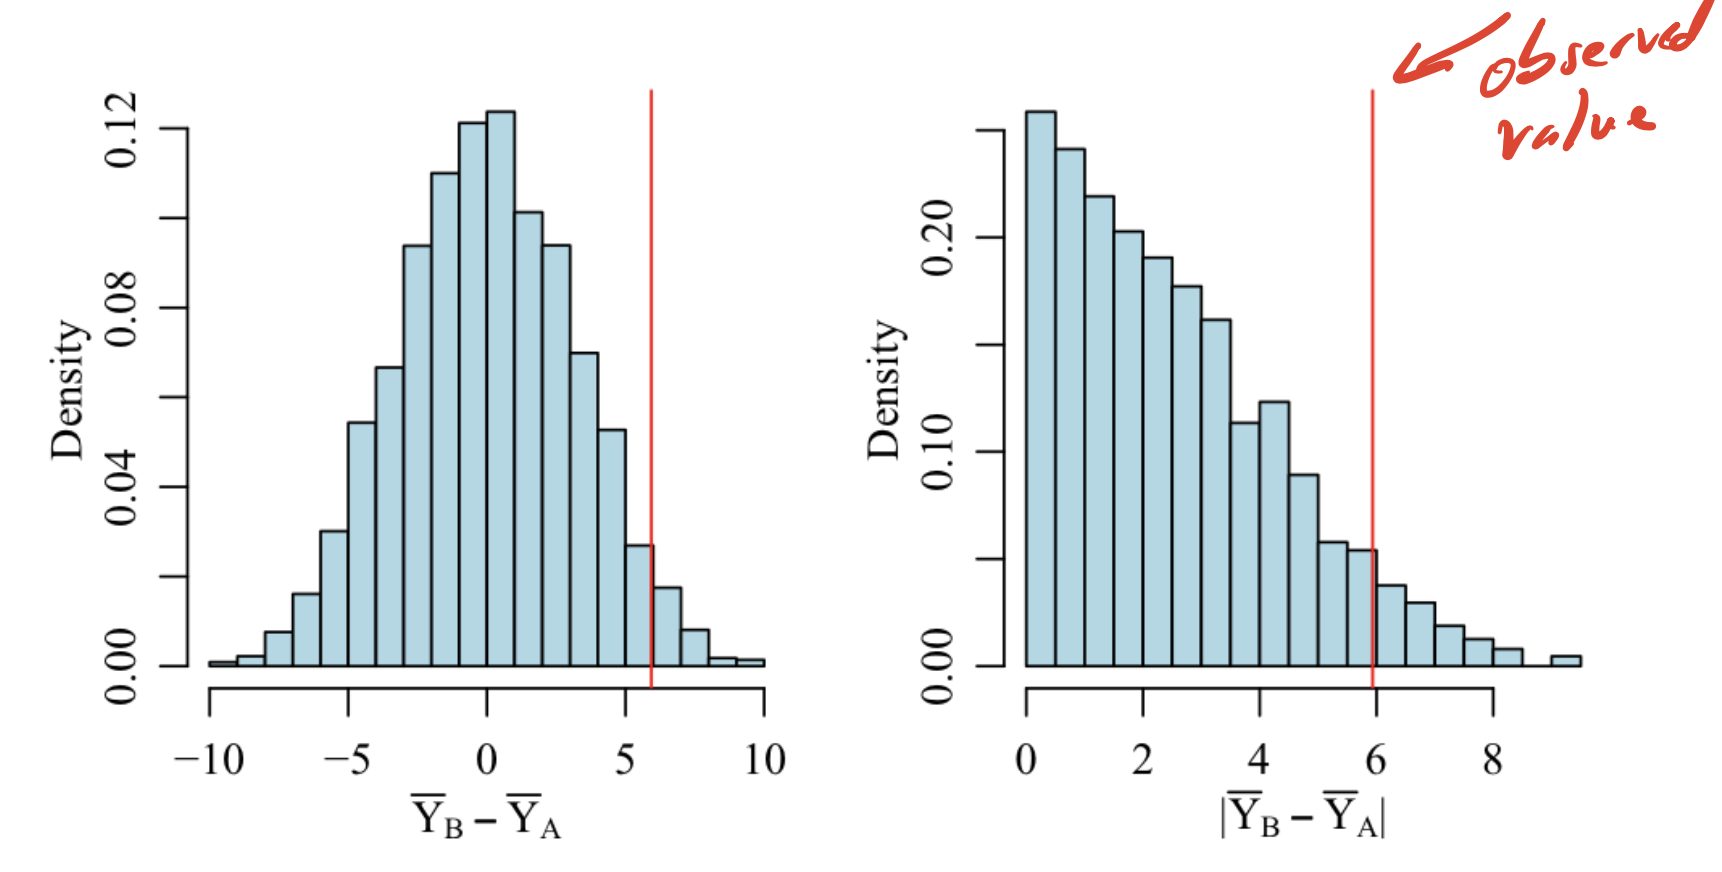
\includegraphics[width=1\textwidth]{fig1.png}
    \textbf{Randomization Null Distribution}
\end{figure}

\section*{Comparing Sample to Null Distribution}
\[
P \left( g(Y_A, Y_B) \geq 5.93 \mid H_0 \right) = 0.056
\quad \textcolor{red}{\text{(kind of unlikely)}}
\]

\textcolor{blue}{This calculation is called the p-value:}
\textcolor{red}{``the prob., under $H_0$, of obtaining a result as or more extreme than the observed result.''}

\subsection*{Basic idea}
\[
\text{small p-value} \quad \rightarrow \quad \text{evidence against } H_0
\]
\[
\text{large p-value} \quad \rightarrow \quad \text{no evidence against } H_0
\]

\subsection*{Approximating a Randomization Distribution}

Enumerating all $\binom{n_A + n_B}{n_A}$ 
possible treatment assignments can be computationally costly.

\subsection*{Instead can do:}

1) randomly simulate a treatment assignment from the population of possible treatment assignments

\noindent 2) compute test statistic given the simulated assignment under \(H_0\)
\[
\textcolor{blue}{\text{Empirical Distribution}} \text{ of } \left\{ \xi_1, \xi_2, \dots, \xi_S \right\} \text{ approximates } H_0
\]
\[
\frac{\#(gs \geq g_{\text{obs}})}{S} \approx P \left( g(Y_A, Y_B) \geq g_{\text{obs}} \mid H_0 \right)
\]
\begin{figure}[H]
    \centering
    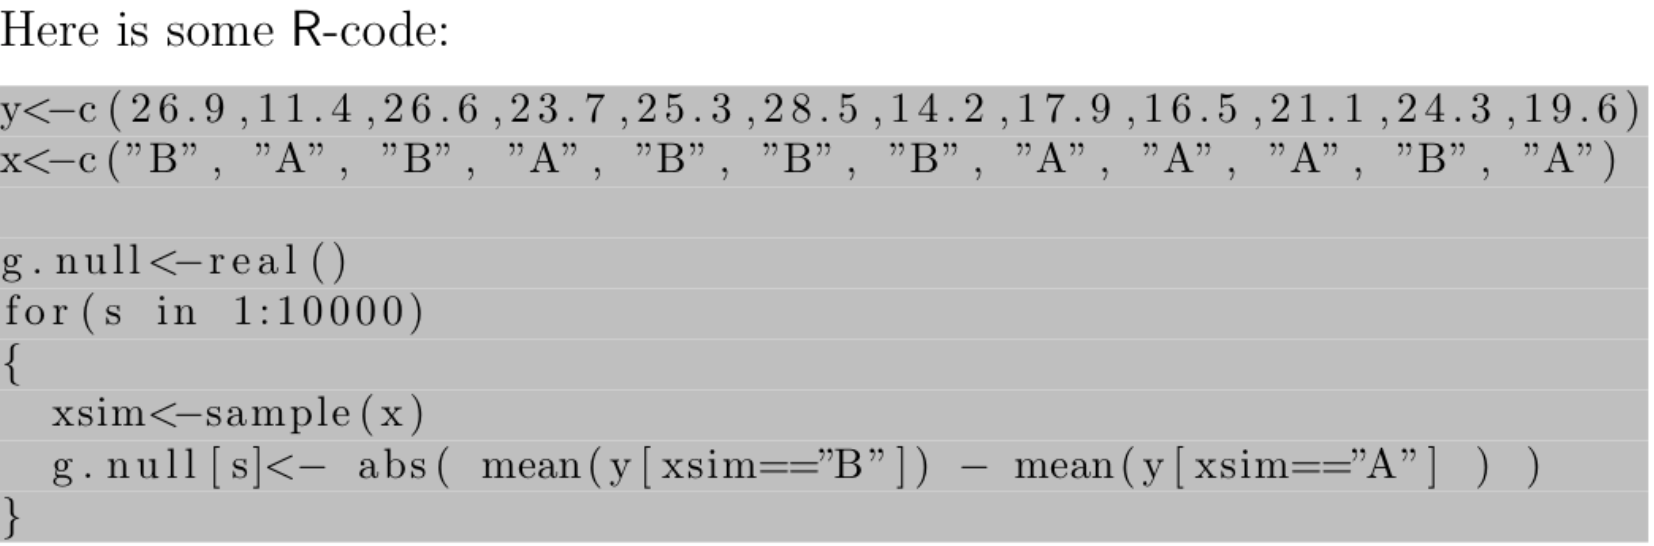
\includegraphics[width=1\textwidth]{fig2.png}
\end{figure}

\subsection*{Note:}

Hypothesis testing is sensitive to the alternative hypothesis \(H_1\).

For example, could use t-test (\textcolor{blue}{sensitive to mean differences})\textcolor{red}{(will see next)} or Kolmogorov-Smirnov (\textcolor{blue}{sensitive to dist. differences}) test as two different test statistics. Can get different conclusions.

\subsection*{Basics of Decision Making}
\begin{figure}[H]
    \centering
    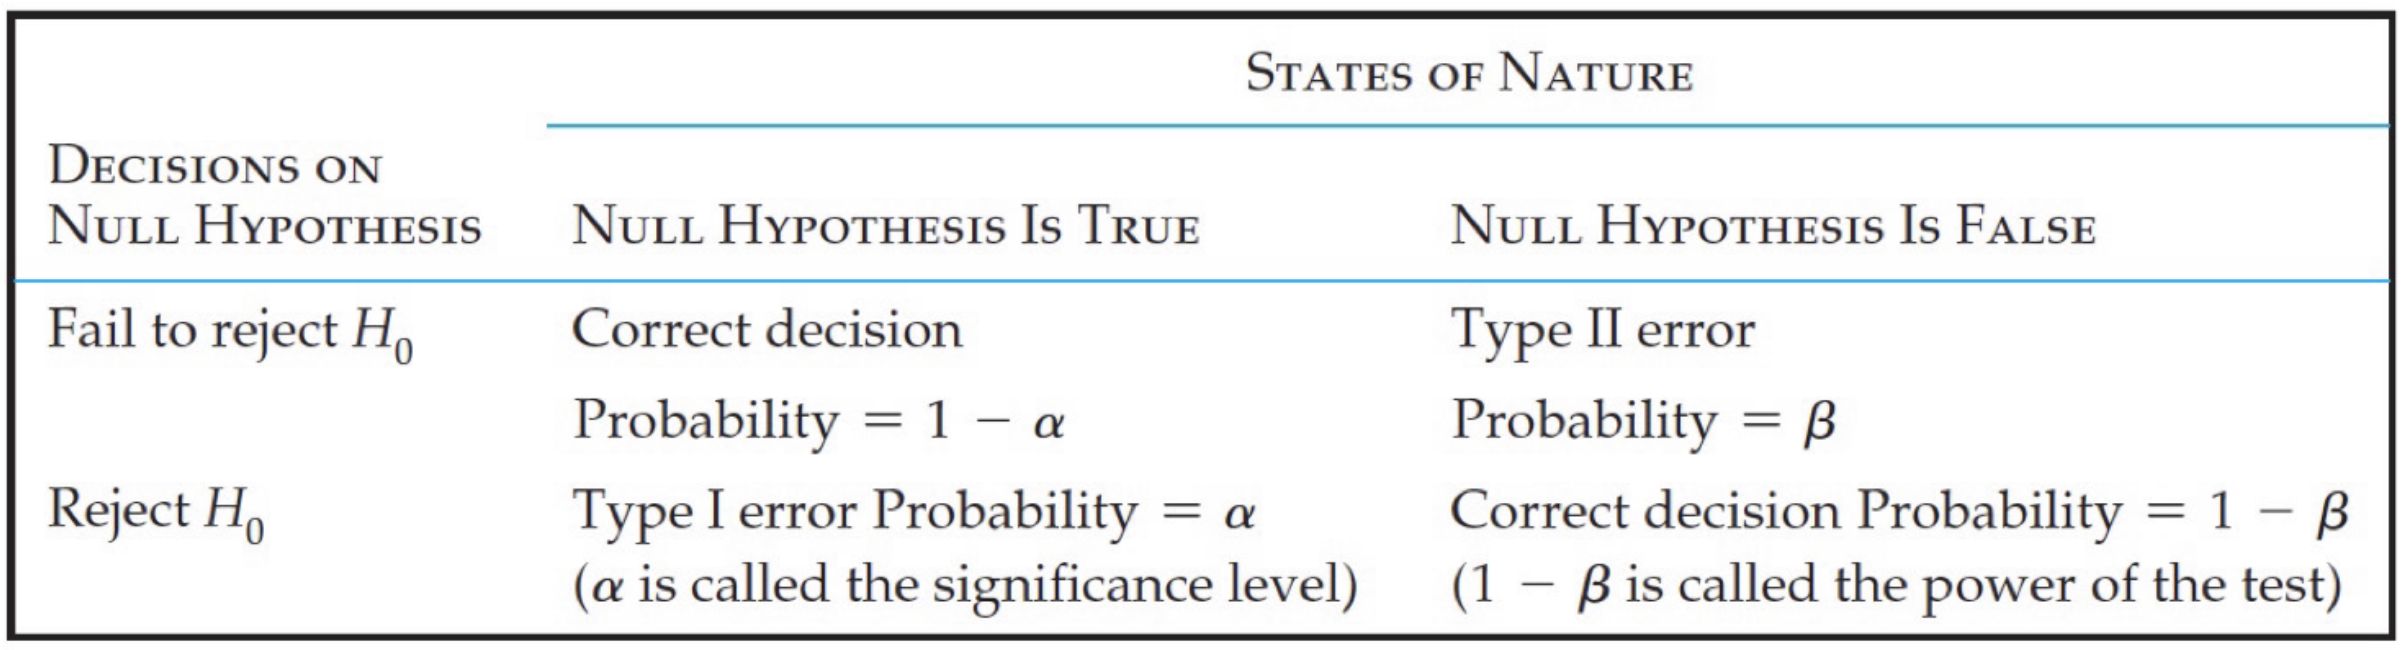
\includegraphics[width=1\textwidth]{fig3.png}
\end{figure}

\textbf{Decision procedure}

\noindent 1. Compute p-value \\ 
2. Reject \( H_0 \) if p-value is small - typical to set this as \( \alpha \)
\vspace{0.5cm}

\noindent This procedure is called a \textcolor{blue}{level \( \alpha \) test.}

\noindent Controls \textcolor{blue}{pre-experimental} probability of a Type I error or for a series of \textcolor{blue}{(independent)} experiments, controls the \textcolor{blue}{type I error rate.}
\[
P(\text{Type I error} \mid H_0) = P(\text{Reject } H_0 \mid H_0) = P(\text{p-value} \leq \alpha \mid H_0) = \alpha
\]
\noindent \textcolor{red}{(Some hidden theory about the distribution of the p-value under \( H_0 \))}

\section*{Single Experiment Interpretation}

If you use a level \( \alpha \) test when \( H_0 \) is true, the probability is \( \alpha \) that you will erroneously reject \( H_0 \).

\subsection*{Many Experiments Interpretation}

If level \( \alpha \) tests are used in a large population of experiments, then \( H_0 \) will be declared false in \( (100 \times \alpha) \% \) of them in which \( H_0 \) is true.

\noindent   \textcolor{green}{\textbf{Note:}
\[
P(\text{Reject } H_0 \mid H_0 \text{ false}) = 1 - \beta = \text{power}
\]}
\textcolor{red}{need to be more specific on what this means to calculate power.}

\textcolor{blue}{[will see more later]}

\noindent - \( \alpha \) and \( \beta \) cannot be simultaneously minimized, so there is a trade-off between \( \alpha \) and \( \beta \).

\noindent - Usually, fix \( \alpha \) and try to minimize \( \beta \) (or equivalently maximize \( 1 - \beta \)).
\begin{figure}[H]
    \centering
    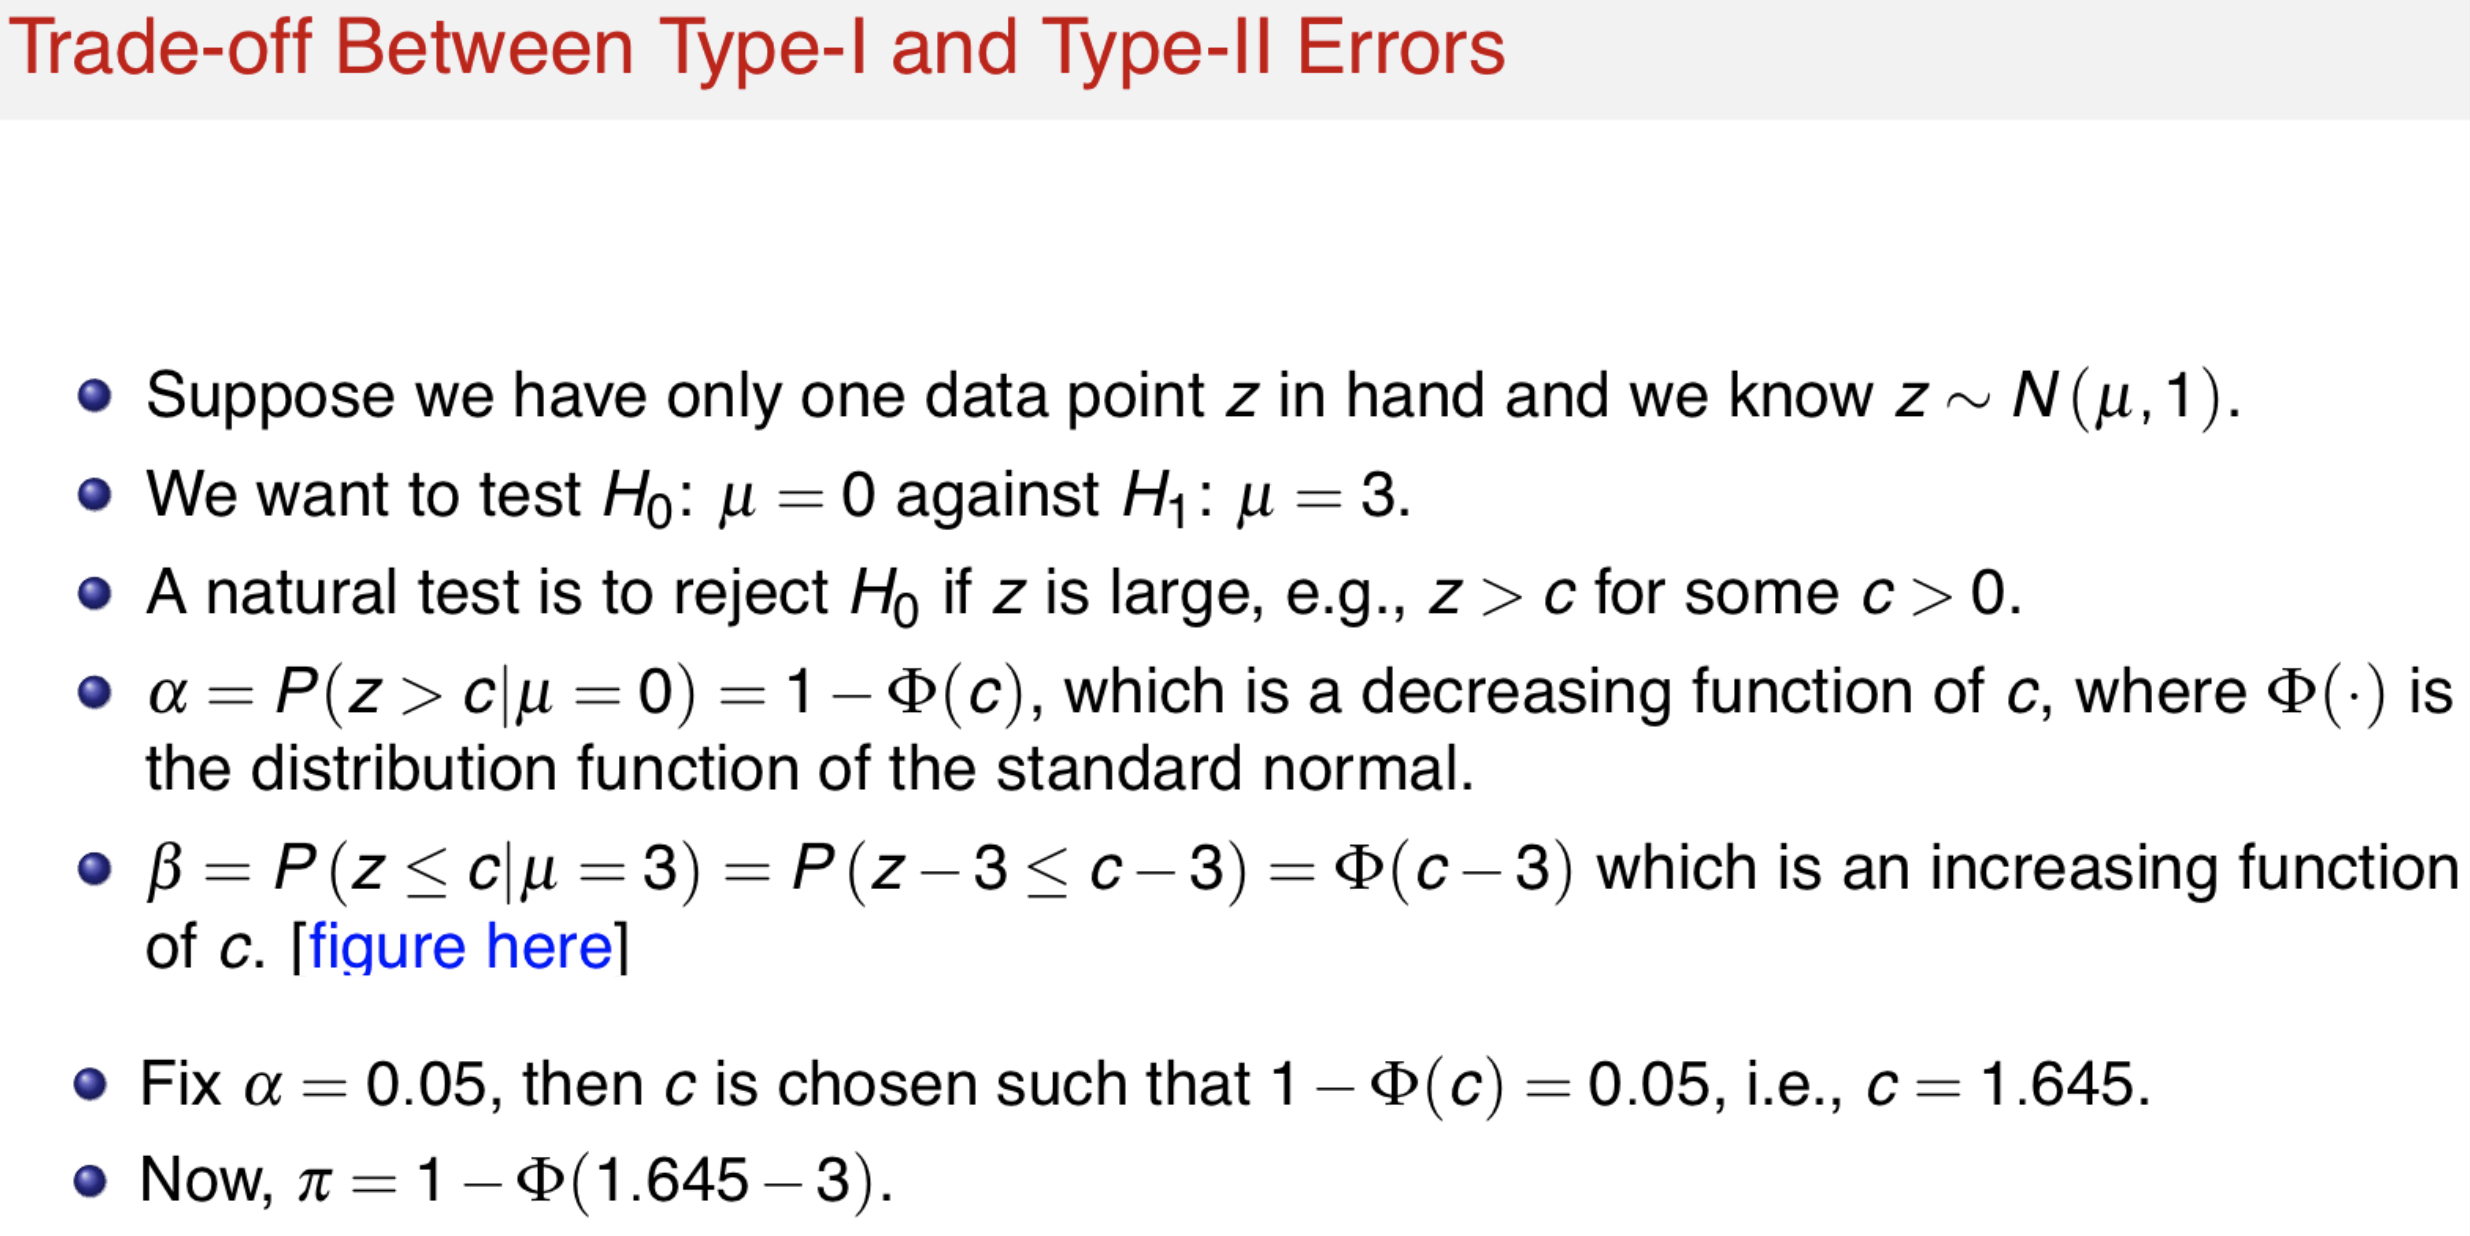
\includegraphics[width=1\textwidth]{fig4.png}
\end{figure}

\begin{figure}[H]
    \centering
    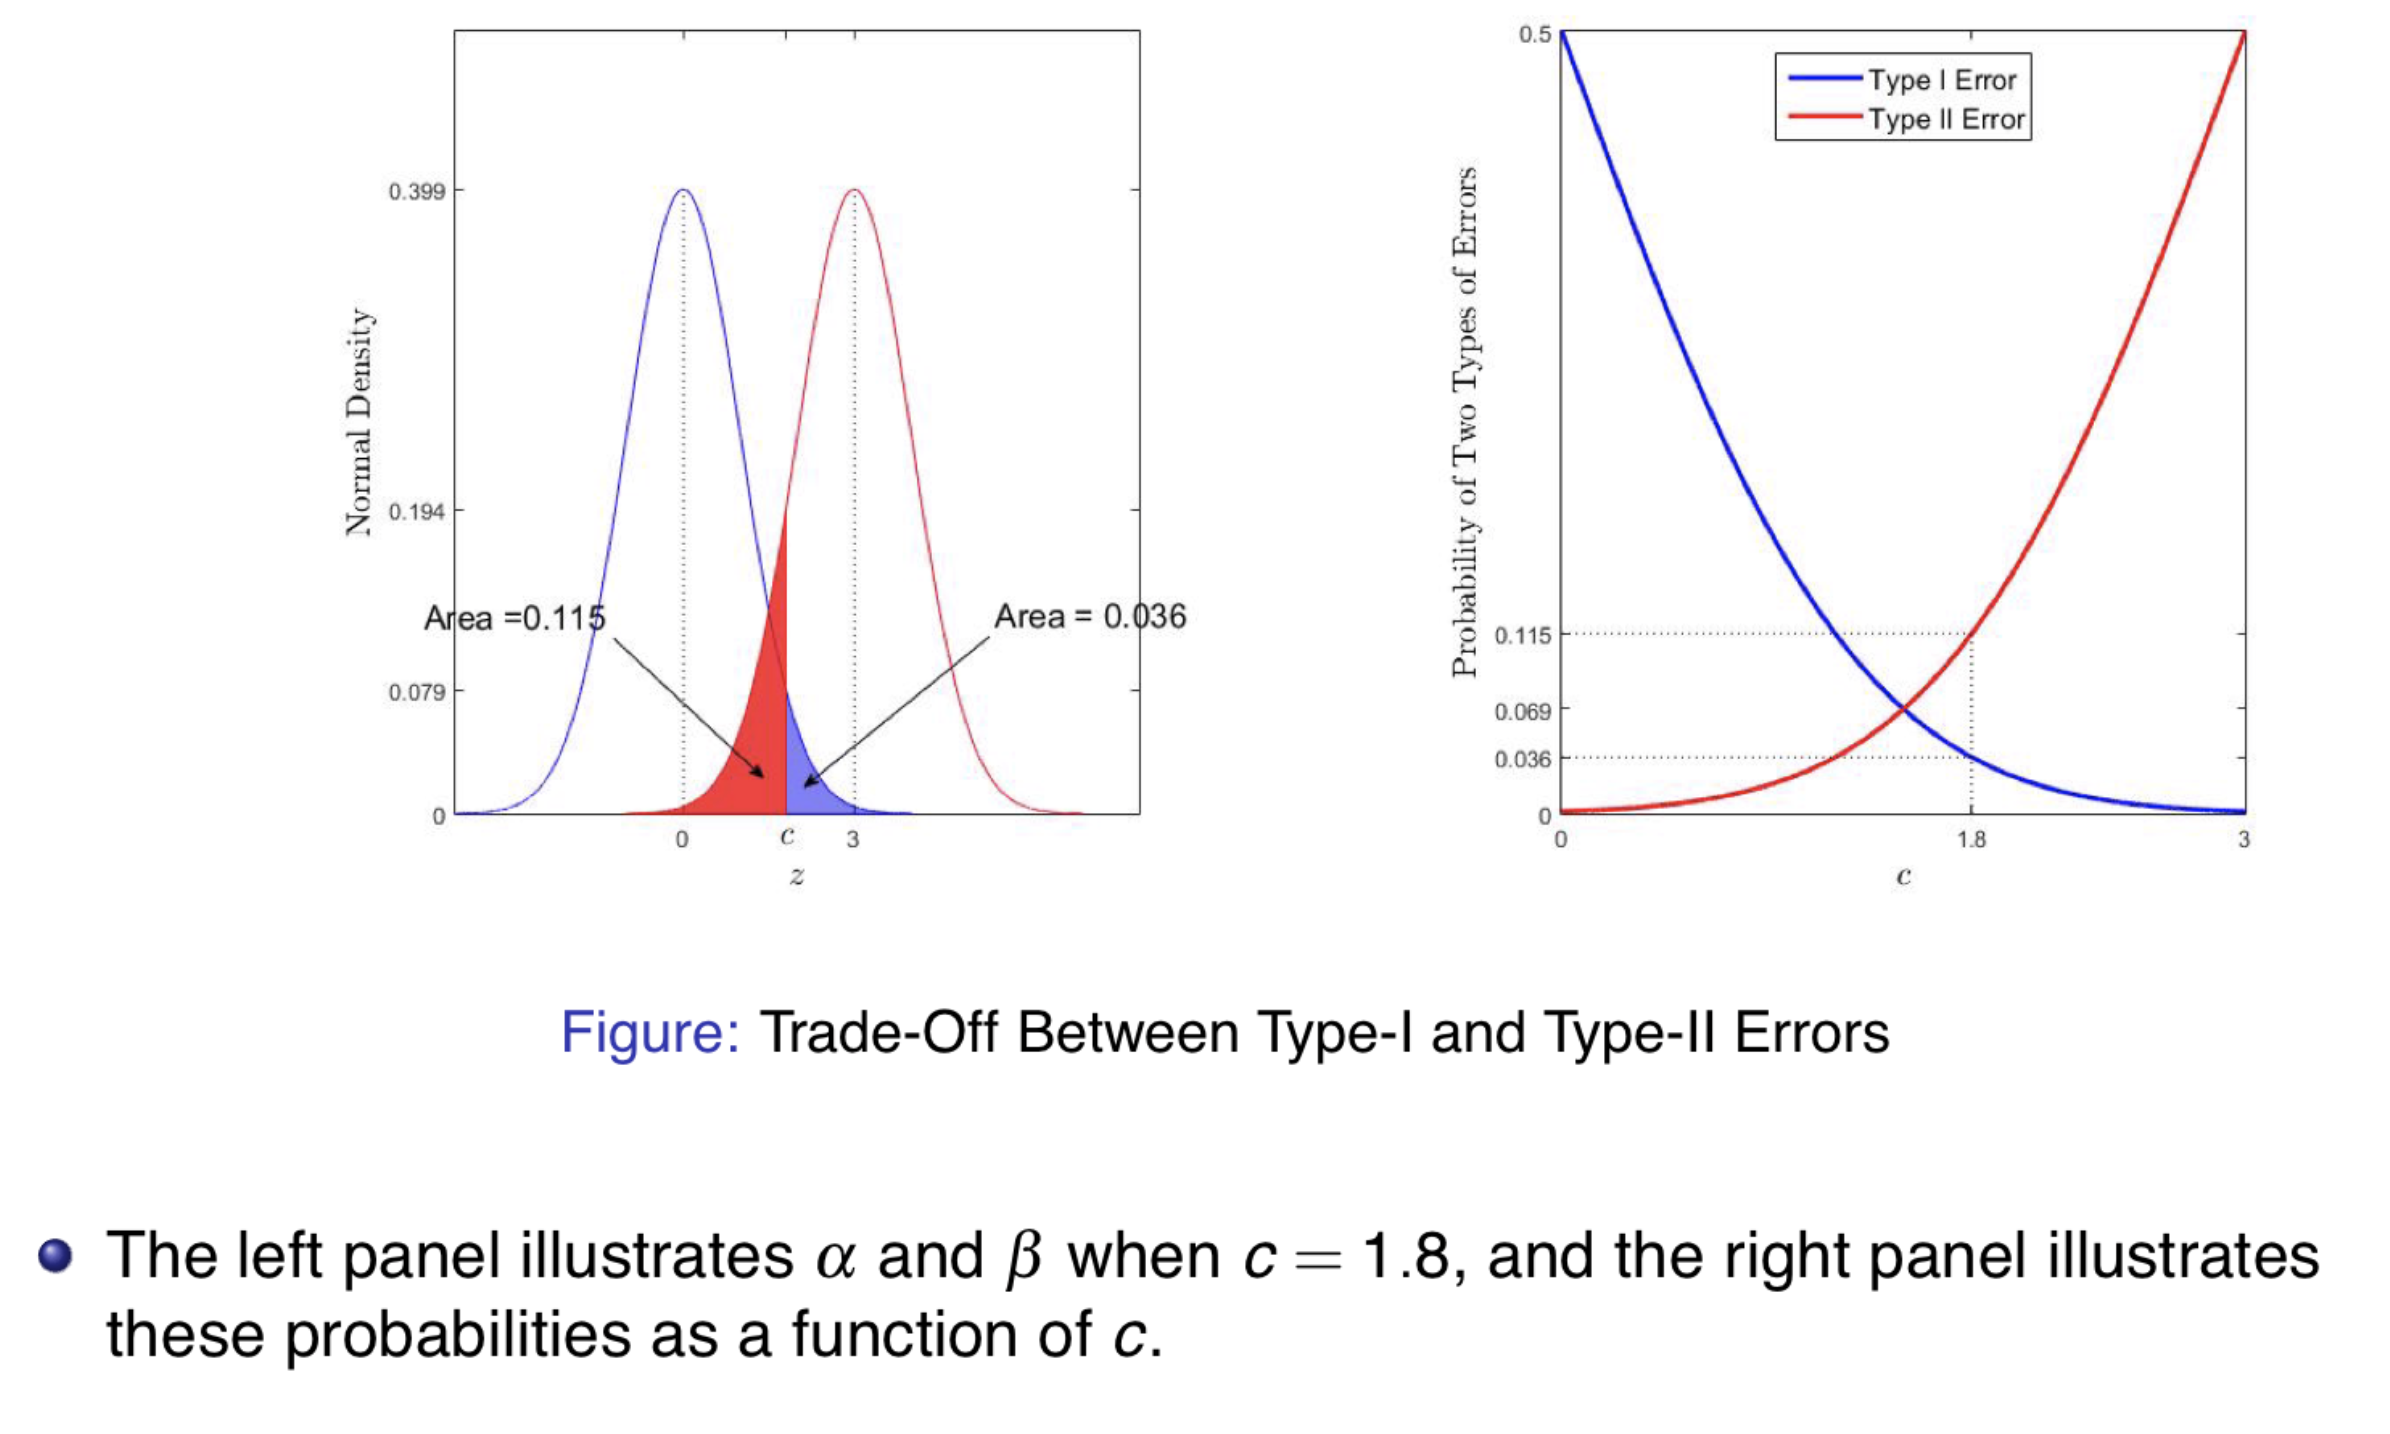
\includegraphics[width=1\textwidth]{fig5.png}
\end{figure}



\end{document}

